% !TEX root = ../main.tex
% !TEX program = xelatex
\section{问题二的模型建立与求解}
\subsection{供需预测与近期误差准备}
问题二需要在当天供需尚未确定时提前订电。候选包括历史分项预测、岭回归\cite{hoerl}和提升树\cite{friedman}。历史参照预测方法\cite{hyndman}便于利用负载的星期规律和光伏的近期变化，解释供需判断的来源；后两者则可利用更多特征描述线性或非线性关系。

预测之后，还需要决定如何承担偏差带来的购电损失。因此，本文采用\textbf{历史分项预测、近期加权准备与跨日线性规划}，根据近期缺口误差设置准备，再结合储能余量确定订单，以减少预测不足时的高价补购。

\subsubsection*{（1）负载与光伏分别预测}
负载取过去四个相同星期位置的同刻平均，光伏取最近七天的同刻平均：
\begin{equation}
\widehat L_{d,k}=\frac14\sum_{j=1}^{4}L_{d-7j,k},\qquad
\widehat P^{PV}_{d,k}=\frac17\sum_{j=1}^{7}P^{PV}_{d-j,k}.
\label{eq:q2_forecast}
\end{equation}
四周同星期数据保留负载的星期规律，并平滑单日波动；七天光伏数据反映近期发电水平。上述窗口结合1月份的方案比较确定，历史不足时对当时已有的对应记录取平均。

跨日规划所需的次日负载，按次日星期位置选取历史；次日光伏仍参考当前零点以前最近七天的数据。两天预测均以\textbf{当前零点}为信息截止点，不使用未来真实值，也不引入附件3的光伏预报。

\subsubsection*{（2）根据近期误差设置准备}
连续低估负载或高估光伏，会使电池不断补充缺口，最终可能触及库存下限。为此，定义历史净需求预测误差：
\begin{equation}
\varepsilon_{i,k}=\left[(L_{i,k}-P^{PV}_{i,k})-(\widehat L_{i,k}-\widehat P^{PV}_{i,k})\right]\Delta t.
\label{eq:q2_error}
\end{equation}
正值表示实际缺口大于预测。历史预测按当时能够获得的信息形成。

将一天分为六个4小时区间，收集最近28天同一区间的误差。设 $\mathcal H_{d,g}$ 为第 $d$ 天零点可用的第 $g$ 组记录，对历史误差赋予权重：
\begin{equation}
\omega_{d,i,k}=\frac{\beta^{d-1-i}}{\displaystyle\sum_{(j,u)\in\mathcal H_{d,g}}\beta^{d-1-j}},\qquad (i,k)\in\mathcal H_{d,g}.
\label{eq:q2_weight}
\end{equation}
较新的记录权重更高，使准备量跟随近期变化。按误差排序并累计权重，取相应分位：
\begin{align}
F_{d,g}(u)&=\sum_{(i,k)\in\mathcal H_{d,g}}\omega_{d,i,k}\mathbf1(\varepsilon_{i,k}\le u),\label{eq:q2_cdf}\\
b_{d,k}&=\max\left\{0,\inf\{u:F_{d,g(k)}(u)\ge\alpha\}\right\}.\label{eq:q2_reserve}
\end{align}
其中，\textbf{$\alpha$控制准备程度，$\beta$控制旧误差的衰减速度}。本文均取0.7，但二者作用不同：70\%分位是误差分布中的位置，不是直接增加70\%的购电量，也不是供电可靠率。

取 $\beta=0.7$ 时，历史权重约每两天减半，既突出近期变化，也保留此前记录。较大的 $\beta$ 保留更多早期误差，在本题比较中反而增加费用；继续减小则会使权重集中于少数日期，更容易受单日异常影响。结合1月8—31日的前期比较与评价期费用，本文选择0.7，兼顾近期响应与历史平滑。全年费用比较覆盖0.7、0.8和0.9三档，详见第6.5节。

准备量进入规划净需求后，既可能增加预计缺口，也可能减少计划中的光伏富余，最终购电量仍由储能调度共同决定。

\subsection{跨日购电与储能模型}
只考虑当天，可能使模型在午夜前过早用尽储能。因此，每天零点规划未来48小时，共288个时段，\textbf{只固定当天前144个时段的订单}；次日安排用于辅助当前决策，到次日零点再重新制定。

用 $t$ 连续编号规划时段，含准备量的净需求为
\begin{equation}
N_t=(\widehat L_t-\widehat P^{PV}_t)\Delta t+b_t,\qquad
n_t=\max(N_t,0),\quad a_t=\max(-N_t,0).
\label{eq:q2_net_demand}
\end{equation}
其中，$n_t$ 为计划缺口，$a_t$ 为扣除准备后的预计余量。

\noindent\textbf{约束1：计划供需平衡。}普通订单满足
\begin{equation}
q_t=n_t-z_t+x_t.
\label{eq:q2_purchase}
\end{equation}
以计划购电费用减去期末储电参考价值为目标：
\begin{equation}
\min J=\sum_{t=1}^{288}p_tq_t-\nu S_{288},\qquad \nu=\eta_dp_{00:00}.
\label{eq:q2_objective}
\end{equation}
内部1 kWh电量能够向负载输出约 $\eta_d$ kWh，因此按零点电价赋予参考价值。该项用于减轻规划末端的影响，不作为售电收入，也不从实际账单中扣除。

\noindent\textbf{约束2：储能运行限制。}功率、储电递推与容量限制沿用式\eqref{eq:q1_power_constraint}—\eqref{eq:q1_soc_bound}，光伏充电上限改为预计余量 $a_t$，放电上限采用计划缺口 $n_t$。

\noindent\textbf{约束3：初始库存与跨日衔接。}取 $S_0=S_{d,0}$，日末实际余电传递至次日，不再要求每日首尾相等。

规划通过准备量应对补购风险，实际效果按普通电费与紧急电费之和评价。

\subsection{模型求解与实际运行}
岭回归与提升树候选由scikit-learn实现\cite{pedregosa}，各策略按以下步骤连续运行。

\noindent\textbf{步骤1：形成供需预测与准备量。}每天零点，按第6.1节处理已有历史，形成未来48小时的供需判断。

\noindent\textbf{步骤2：求解跨日计划。}从当前实际库存开始，采用HiGHS求解，只固定当天订单。

\noindent\textbf{步骤3：按实际供需执行。}日内订单保持不变，储能根据实际供需充放电。

设某时段实际负载电量为 $l$，光伏电量为 $v$，普通订单为 $q$，时段开始时内部储电量为 $S$。供电不足时，先由电池补充，再紧急购买剩余缺口：
\begin{align}
D&=\max(l-v-q,0),\label{eq:q2_actual_deficit}\\
z^{\mathrm{act}}&=\min\{D,P_{\max}\Delta t,\eta_d(S-S_{\min})\},\qquad e=D-z^{\mathrm{act}}.\label{eq:q2_emergency}
\end{align}
存在余电时，在容量与充电功率允许范围内储存：
\begin{equation}
c^{\mathrm{act}}=\min\left\{\max(v+q-l,0),P_{\max}\Delta t,\frac{S_{\max}-S}{\eta_c}\right\}.
\label{eq:q2_actual_charge}
\end{equation}
充电优先使用富余光伏，再使用普通订单余量，内部储电量更新为
\begin{equation}
S^{\mathrm{next}}=S+\eta_cc^{\mathrm{act}}-\frac{z^{\mathrm{act}}}{\eta_d}.
\label{eq:q2_actual_soc}
\end{equation}
\noindent\textbf{步骤4：结算并衔接次日。}未能使用或储存的普通订单仍需付费，未利用光伏不计售电收益。每日实际费用及跨日衔接为
\begin{equation}
C_d=\sum_{k=1}^{144}\left(p_kq_{d,k}+5p_ke_{d,k}\right),\qquad S_{d+1,0}=S_{d,144}.
\label{eq:q2_daily_cost}
\end{equation}
运行从1月1日零点的6000 kWh开始，首日采用问题一的购电安排。实测序列缺少首个00:00—00:10区间，仅该段借用附件1零点供需作启动参考，不作为实测值或预测训练标签；此后使用附件2的连续实测数据。

1月份用于历史积累、前期参数比较和库存衔接。2月1日得到8592.69 kWh，作为各候选及问题三、四的共同评价起点，此后各策略继承自身前一天的实际余电。2—12月用于连续运行评价，也为近期加权方法的选择提供误差诊断依据。各日购电决策均只使用当时已获得的信息。

\subsection{方案比较与运行结果}
\subsubsection*{（1）误差准备的节费作用与方案比较}
统一电价、设备参数、初始库存、规划长度与实际供电规则，比较2025年2月1日至12月31日共334天的实际费用，结果见表~\ref{tab:q2_model_compare}。

\begin{table}[!htbp]
\centering
\caption{不同方案的334天实际购电费用}
\label{tab:q2_model_compare}
\begin{tabular}{lccc}
\hline
方案 & 普通电费/万元 & 紧急电费/万元 & 总电费/万元 \\
\hline
历史分别预测，无误差准备
& 1218.58 & 374.70 & 1593.28 \\
分别岭回归，无误差准备
& 1210.27 & 446.88 & 1657.15 \\
分别提升树，无误差准备
& 1218.25 & 343.71 & 1561.96 \\
历史分别预测，等权误差准备
& 1295.99 & 107.05 & 1403.04 \\
\textbf{历史分别预测，近期加权准备}
& 1297.96 & 60.43 & \textbf{1358.38} \\
\hline
\end{tabular}
\end{table}

表中首先比较不设置准备的三种预测策略，再考察历史分项预测加入准备后的效果。

\begin{samepage}
最终方案较无准备的历史预测方案降低总费用约14.74\%。本题以实际购电费用评价预测、误差准备与储能调度组成的完整策略。历史分项预测利用负载的星期规律和光伏的近期变化，近期加权准备进一步缓冲预测偏差，两者与跨日规划结合后，在本次候选比较中取得最低总费用。
\par\end{samepage}

与等权准备相比，\textbf{近期加权以约1.97万元的新增普通电费，减少约46.63万元的紧急电费，净节省44.66万元}，降幅3.18\%。统一分位数计算方式后，仍节省约44.54万元，说明节费主要来自历史误差权重的调整。

这一组合让准备量跟随近期缺口变化，以适量普通购电减少更昂贵的临时补购，体现了预测与调度共同安排的优势。

\subsubsection*{（2）评价期与指定日期结果}
最终总购电费用为\textbf{13583810.84元}，其中普通电费12979560.57元、紧急电费604250.27元。完整10分钟结果保存于\texttt{result2.xlsx}。其中，计划购电表的全天购电量与费用只计普通订单，紧急购电另表列示；论文中的总费用为普通电费与紧急电费之和。

按月比较，11个月的费用均低于等权准备方案，6月和12月的节省较为明显，说明费用优势覆盖了不同季节。指定日期的结果见表~\ref{tab:q2_specified_purchase}、表~\ref{tab:q2_storage}及紧急购电表。

\begin{table}[!htbp]
\centering
\caption{指定日期的计划购电及全天费用}
\label{tab:q2_specified_purchase}
\begin{tabular}{lrrrr}
\hline
项目 & 3月20日 & 6月21日 & 9月23日 & 12月21日 \\
\hline
10:00--10:10
& 0.00 & 0.00 & 0.00 & 0.00 \\
12:00--12:10
& 610.16 & 0.00 & 484.48 & 943.63 \\
14:00--14:10
& 0.00 & 0.00 & 0.00 & 0.00 \\
16:00--16:10
& 434.90 & 116.65 & 453.86 & 798.03 \\
18:00--18:10
& 716.29 & 437.88 & 826.38 & 742.86 \\
20:00--20:10
& 0.00 & 0.00 & 5.90 & 0.00 \\
全天计划购电量/kWh
& 64232.05 & 40298.69 & 68385.07 & 95446.27 \\
全天紧急购电量/kWh
& 329.52 & 0.00 & 6.38 & 0.00 \\
全天购电合计/kWh
& 64561.57 & 40298.69 & 68391.44 & 95446.27 \\
普通电费/元
& 39469.74 & 22323.80 & 42730.05 & 61249.77 \\
紧急电费/元
& 2298.74 & 0.00 & 43.00 & 0.00 \\
总电费/元
& 41768.47 & 22323.80 & 42773.04 & 61249.77 \\
\hline
\end{tabular}
\end{table}

\begin{table}[!htbp]
\centering
\caption{指定日期的实际充放电量及日首尾储电量}
\label{tab:q2_storage}
\begin{tabular}{llrrrr}
\hline
时间段 & 项目 & 3月20日 & 6月21日 & 9月23日 & 12月21日 \\
\hline
00:00--04:00 & 充电
& 1504.96 & 309.75 & 1739.22 & 1830.47 \\
& 放电
& 185.93 & 229.12 & 2.78 & 227.55 \\

04:00--08:00 & 充电
& 1138.95 & 286.60 & 53.65 & 1476.38 \\
& 放电
& 4670.35 & 1949.50 & 5934.88 & 729.24 \\

08:00--12:00 & 充电
& 5327.26 & 10134.27 & 4409.06 & 4706.14 \\
& 放电
& 3265.56 & 0.00 & 2387.94 & 8254.51 \\

12:00--16:00 & 充电
& 4465.10 & 21.43 & 6147.58 & 8347.54 \\
& 放电
& 369.53 & 0.00 & 521.04 & 2318.98 \\

16:00--20:00 & 充电
& 169.64 & 115.05 & 221.91 & 19.45 \\
& 放电
& 5340.10 & 5107.80 & 4920.36 & 4873.96 \\

20:00--24:00 & 充电
& 4438.27 & 8636.77 & 8446.30 & 8360.50 \\
& 放电
& 3424.22 & 3022.72 & 3633.41 & 3626.10 \\
\hline
0:00储电量/kWh & 
& 8919.73 & 3543.84 & 9214.11 & 8886.94 \\
24:00储电量/kWh &
& 5086.49 & 9642.73 & 8796.25 & 8897.44 \\
\hline
\end{tabular}
\end{table}

% Restored from verified Q2 selected_execution.csv.gz; no model rerun.
\begin{table}[!htbp]
\centering
\caption{问题二指定日期发生紧急购电的时段及电量}
\label{tab:q2_emergency_purchase}
\begin{tabular}{llr}
\toprule
日期 & 时间段 & 紧急购电量/kWh \\
\midrule
3月20日 & 20:40--20:50 & 329.52 \\
9月23日 & 20:30--20:40 & 6.38 \\
\bottomrule
\end{tabular}
\end{table}


6月21日和12月21日均未发生紧急购电，未列出的时段紧急购电量为零。
指定时段订单与充放电量的单位均为kWh；全天合计由完整144个时段汇总。充放电按设备外侧计量，库存按内部电量计量。

\subsubsection*{（3）储能对预测偏差的缓冲}

以3月20日为例，储能补足了大部分订单与实际需求之间的缺口。但20:40开始时内部电量仅剩1622.06 kWh，继续放电触及1200 kWh下限后，仍有329.52 kWh需要紧急购买。

6月21日白天光伏充足，电池能够储存余电并在后续释放，全天未发生紧急购电。

\begin{samepage}
两个日期说明，\textbf{缓冲能力取决于缺口出现时的库存与放电能力}，不能仅由全天供需总量判断。
\par\end{samepage}

\subsection{参数检验与风险分析}

\begin{figure}[!htbp]
    \centering
    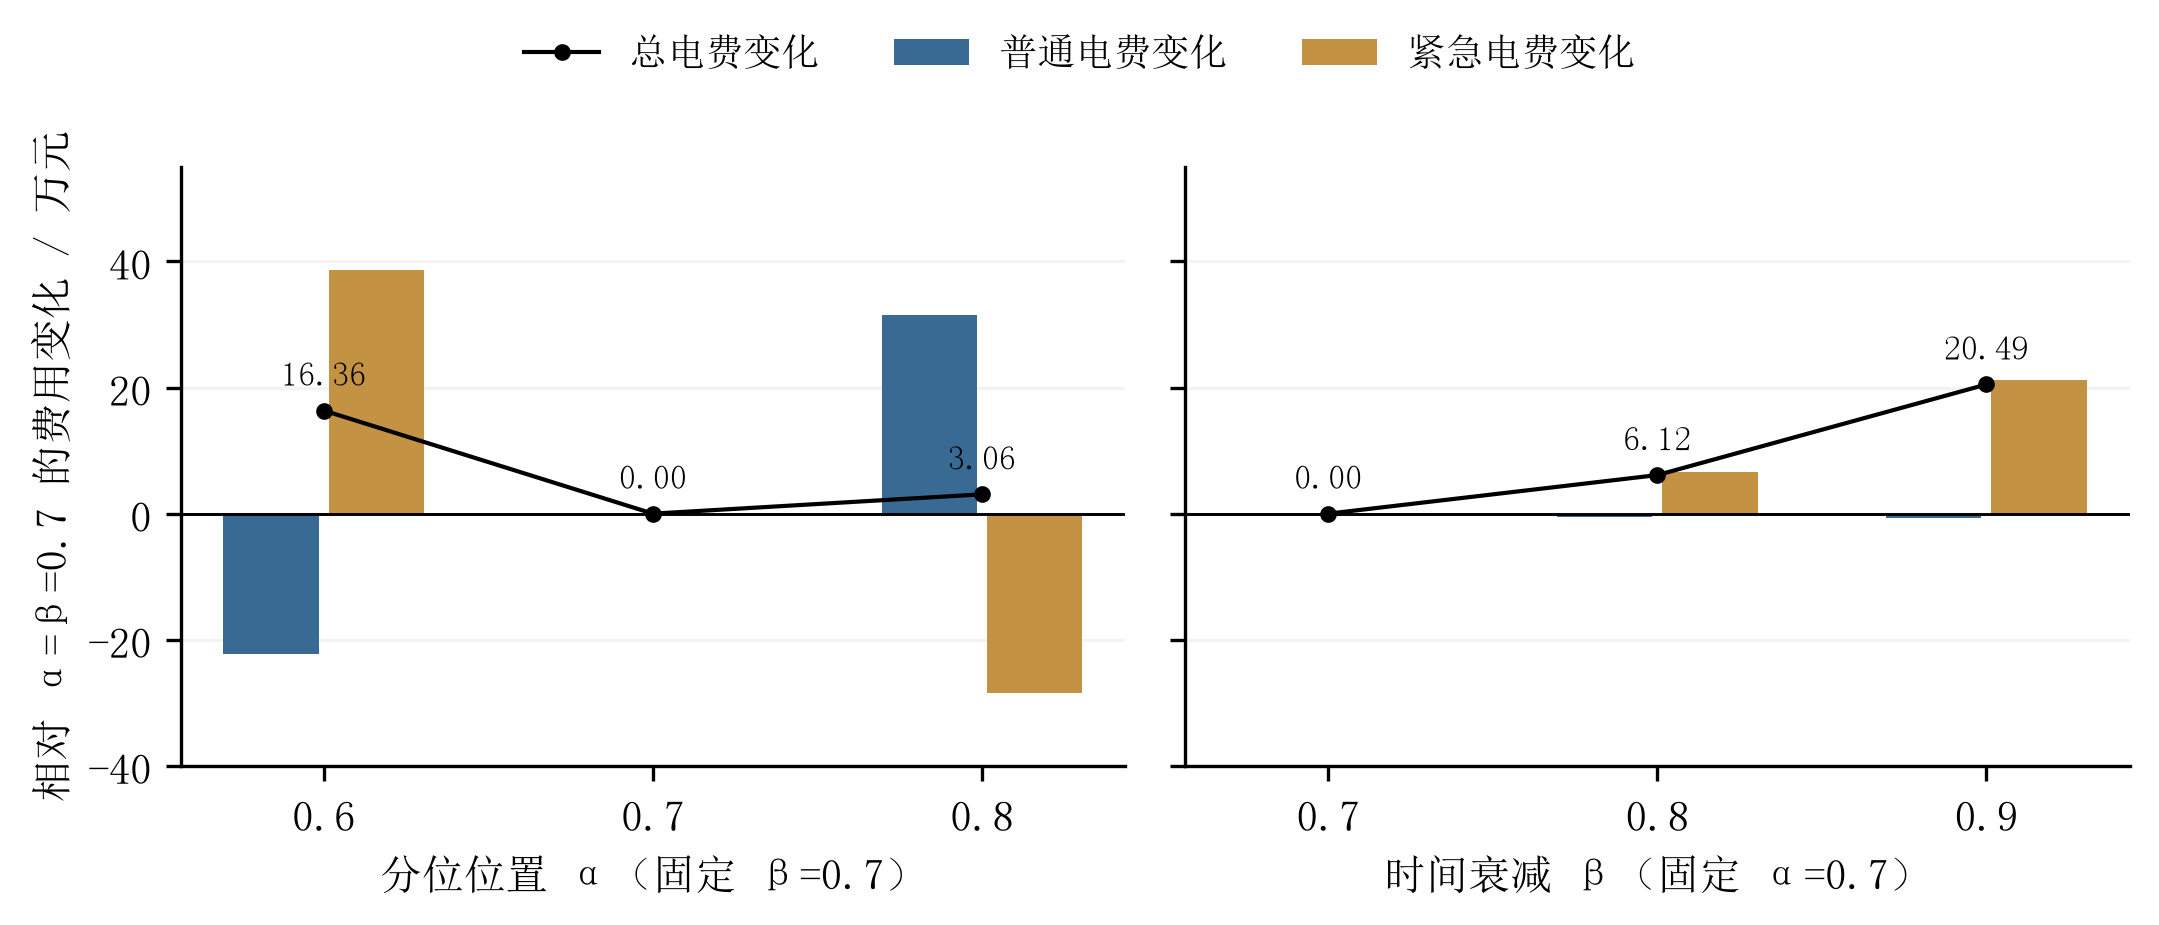
\includegraphics[width=0.82\textwidth]{fig/sensitivity.png}
    \caption{准备程度与近期权重对购电费用的影响}
    \label{fig:q2_sensitivity}
\end{figure}

如图~\ref{fig:q2_sensitivity}所示，固定 $\beta=0.7$，将分位 $\alpha$ 提高至0.8后，紧急购电天数由156天降至102天，但新增普通电费超过紧急电费的节省，总费用上升约3.06万元；降至0.6时，准备不足使总费用上升约16.36万元。

固定 $\alpha=0.7$，将 $\beta$ 提高至0.8和0.9，总费用分别增加约6.12万元和20.49万元。上述比较表明，两个参数取0.7能够较好地兼顾近期响应和购电准备，平衡两类费用。

48小时规划将最长连续紧急补购时间由340分钟缩短至200分钟，并保留更多期末储电，评价期费用仅增加3215.61元。因此，本文以较小的费用代价改善跨日衔接，保留48小时规划。去除期末储电参考价值后，总费用不变，说明节费结果不依赖该项。

从历史误差中选取连续三天的不利片段，构造持续低估负载、高估光伏及两者叠加的情景，保持实际供需不变。近期加权方案仍比等权准备节省3.09\%—3.52\%，保持了总费用优势。其中，持续高估光伏带来的费用增幅略大于等权方案，后续可重点加强对连续光伏偏差的识别。
